% Created 2019-07-12 Fri 17:23
% Intended LaTeX compiler: pdflatex
\documentclass[11pt]{article}
\usepackage[utf8]{inputenc}
\usepackage[T1]{fontenc}
\usepackage{graphicx}
\usepackage{grffile}
\usepackage{longtable}
\usepackage{wrapfig}
\usepackage{rotating}
\usepackage[normalem]{ulem}
\usepackage{amsmath}
\usepackage{textcomp}
\usepackage{amssymb}
\usepackage{capt-of}
\usepackage{hyperref}
\usepackage{lmodern}
\usepackage{minted}
\usepackage{parskip}
\usemintedstyle{emacs}
\newminted{common-lisp}{fontsize=\footnotesize}
\author{adam}
\date{\today}
\title{}
\hypersetup{
 pdfauthor={adam},
 pdftitle={},
 pdfkeywords={},
 pdfsubject={},
 pdfcreator={Emacs 25.2.2 (Org mode 9.2.1)},
 pdflang={English}}
\begin{document}

\tableofcontents


\section{[843] Guess the Word}
\label{sec:orgd790762}
\url{https://leetcode.com/problems/guess-the-word/description/}

\begin{minted}[frame=lines,fontsize=\scriptsize,linenos]{code}
algorithms
Hard (41.56%)
Total Accepted:    13.4K
Total Submissions: 32.2K
Testcase Example:
'"acckzz"\n["acckzz","ccbazz","eiowzz","abcczz"]\n10'
\end{minted}

This problem is an \textbf{interactive problem} new to the LeetCode platform.

We are given a word list of unique words, each word is 6 letters long, and
one word in this list is chosen as secret.

You may call master.guess(word) to guess a word. The guessed
word should have type string and must be from the original list with 6
lowercase letters.

This function returns an integer type, representing the number of exact
matches (value and position) of your guess to the secret word.  Also, if your
guess is not in the given wordlist, it will return -1 instead.

For each test case, you have 10 guesses to guess the word. At the end of any
number of calls, if you have made 10 or less calls to master.guess and at
least one of these guesses was the secret, you pass the testcase.

Besides the example test case below, there will be 5 additional test cases,
each with 100 words in the word list.  The letters of each word in those
testcases were chosen independently at random from 'a' to 'z', such that
every word in the given word lists is unique.

\subsection{Example 1:}
\label{sec:org9547464}
\begin{itemize}
\item Input: secret = "acckzz", wordlist = ["acckzz","ccbazz","eiowzz","abcczz"]

\item Explanation:

master.guess("aaaaaa") returns -1, because "aaaaaa" is not in wordlist.

master.guess("acckzz") returns 6, because "acckzz" is secret and has
all 6 matches.

master.guess("ccbazz") returns 3, because "ccbazz" has 3 matches.

master.guess("eiowzz") returns 2, because "eiowzz" has 2 matches.

master.guess("abcczz") returns 4, because "abcczz" has 4 matches.

We made 5 calls to master.guess and one of them was the secret, so we pass
the test case.
\end{itemize}

\section{minimax solution}
\label{sec:org5059eb0}

This is not an attempt to make the most efficient or expedient
solution, but one that appeals to my sense of a minimax problem.

\section{basically idea}
\label{sec:org861c5b7}

My opponent is trying to pick a secret word that will leave me with
least information about the secret's identity.  As the player, I am
trying to pick a guess that maximizes this information.

\section{(max)imizing the (min)imum information}
\label{sec:org43519fe}

One simple gauge of (mis-)information is the amount of remaining words after
each query.  In the picture below,

\begin{center}
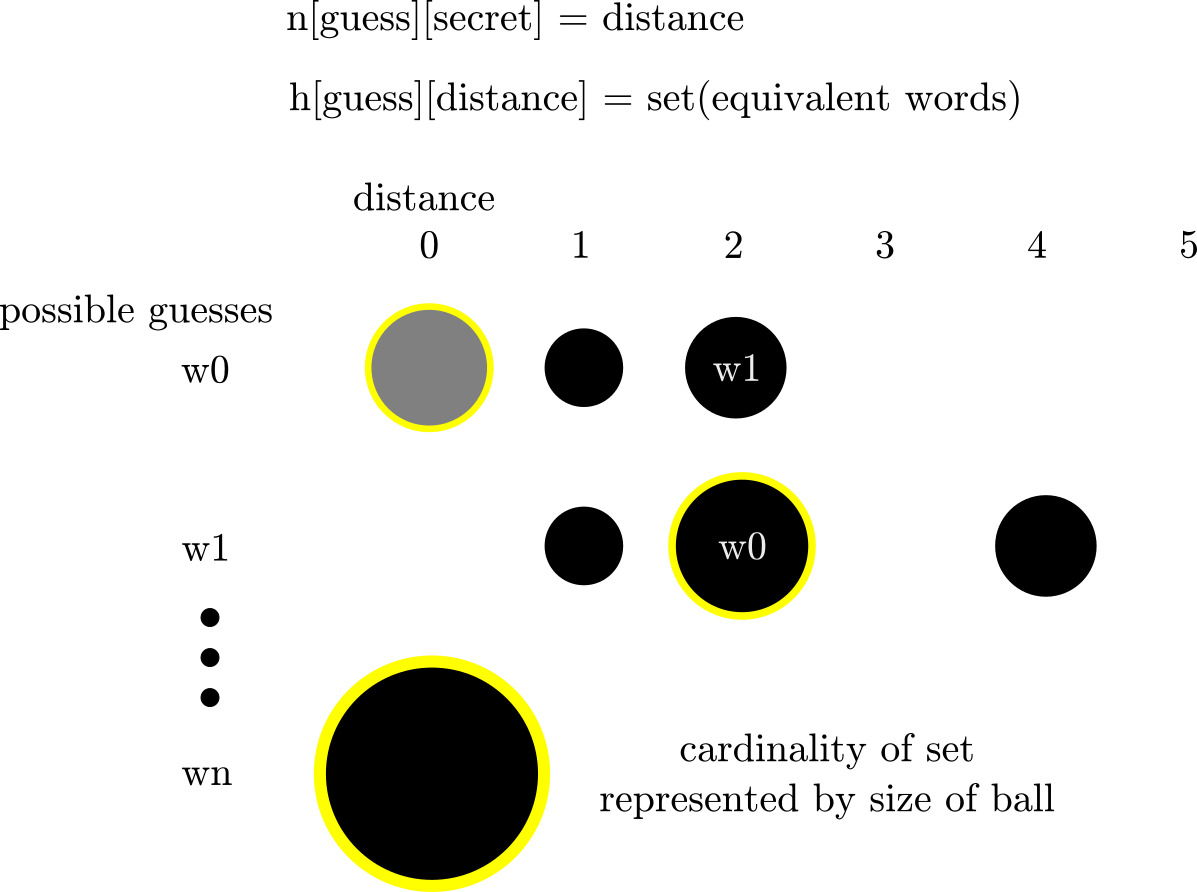
\includegraphics[width=.9\linewidth]{./guess.png}
\end{center}

I represent the number of remaining words as the cardinality of the
set, which is represented by the size of the circle.  The set
represents the number of words that share similar distance to a
particular guess.  \(n(g,s)\) represents the distance between two words,
\(g\) and \(s\) (\(g\) for guess and \(s\) for secret) and \(h(g,n(g,s))\)
represents the set containing all the words that have the same
distance to \(g\).  For example, for \([aab, acb, aac]\), \(n(aab, acb) =
n(aab, aac) = 2\), thus \(h(aab, 2) = {acb, aac}\).  Let \(|h|\) denote the
cardinality of \(h\).

Then for a particular guess, \(g\), my opponent will seek a secret word,
\(s\), such that maximizes \(|h(g, n(g,s))|\) for all posible choices of
\(s\).  This is represented by the yellow outline, ie the smaller the
size of the circle the more I know about the whereabouts of \(s\), so my
opponent chooses the \(s^*(g) = \textrm{argmax}_s |h(g, n(g,s)|\).

The player then has a choice of \(g\), the guess, that maximizes his
information about \(s\), or the smallest circle, so he chooses \(g^* =
\textrm{argmin}_g s^*(g)\).  This is represented by the gray shaded
circle in the picture.

This will result in a smaller set of choices for the following round.
In the code, I perform a \(|h(g, d) \cap G|\) where \(G\) is the
possible set of \(g\)'s, guesses, after each round, rather than
recompute \(h(g, d)\).

\section{code}
\label{sec:orgedd2015}
\begin{minted}[frame=lines,fontsize=\scriptsize,linenos]{python}
from collections import defaultdict


class Solution:

    def near(self, i, j, w):
        ret = sum([x[0] == x[1] for x in zip(w[i], w[j])])
        return ret

    def nearw(self, wi, wj):
        ret = sum([x[0] == x[1] for x in zip(wi, wj)])
        return ret

    def guess(self, select, secret):
        return self.nearw(select, secret)

    def findSecretWord(self, w, master):
        """
        create a "near" list
        """

        h = [None] * len(w)  # keeps the set
        n = [None] * len(w)  # keeps the near matrix
        for i in range(len(h)):
            h[i] = defaultdict(set)
            n[i] = [0] * len(w)

        for i in range(0, len(w) - 1):
            for j in range(i + 1, len(w)):
                nr = self.near(i, j, w)
                n[i][j], n[j][i] = nr, nr
                h[i][nr].add(j)
                h[j][nr].add(i)

        def remaining_choices(select, nr, choices):
            return len(h[select][nr] & choices)

        choices = set(range(len(w)))
        while True:
            max_cost = {}
            if len(choices) > 1:
                for select in choices:
                    cost = {}
                    visited = set()
                    for secret in choices:
                        if select != secret:
                            nr = n[select][secret]
                            if nr not in visited:
                                cost[secret] = remaining_choices(
                                    select, nr, choices)
                                visited.add(nr)
                    # find the max cost among all the secrets
                    max_cost[select] = max(cost.items(), key=lambda x: x[1])
                mcost = {k: v[1] for k, v in max_cost.items()}
                minmax = min(mcost.items(), key=lambda x: x[1])
                selection = minmax[0]
            else:
                selection = list(choices)[0]

            offline = False
            if offline:
                my_secret = w[1]
                my_secret = "hbaczn"
                matches = self.guess(w[selection], my_secret)
                my_secret_index = w.index(my_secret)
                print(
                    ("Secret: {}, Index: {}, " +
                     "Matches: {}, N: {}, |N|: {}").format(
                         my_secret, my_secret_index,
                         n[selection][my_secret_index],
                         h[selection][matches],
                         len(h[selection][matches])))
            else:
                matches = master.guess(w[selection])

            if matches == 6:
                print("found")
                break
            choices = h[selection][matches] & choices

        return w[selection]


test = True
if test:
    s = Solution()
    case = [False] * 1 + [True] + [False] * 1
    master = None
    if case[0]:
        # Example 1:
        secret = "acckzz"
        wordlist = ["acckzz", "ccbazz", "eiowzz", "abcczz"]
        print(s.findSecretWord(wordlist, master))
    if case[1]:
        secret = "hbaczn"
        wordlist = [
            "gaxckt", "trlccr", "jxwhkz", "ycbfps", "peayuf", "yiejjw",
            "ldzccp", "nqsjoa", "qrjasy", "pcldos", "acrtag", "buyeia",
            "ubmtpj", "drtclz", "zqderp", "snywek", "caoztp", "ibpghw",
            "evtkhl", "bhpfla", "ymqhxk", "qkvipb", "tvmued", "rvbass",
            "axeasm", "qolsjg", "roswcb", "vdjgxx", "bugbyv", "zipjpc",
            "tamszl", "osdifo", "dvxlxm", "iwmyfb", "wmnwhe", "hslnop",
            "nkrfwn", "puvgve", "rqsqpq", "jwoswl", "tittgf", "evqsqe",
            "aishiv", "pmwovj", "sorbte", "hbaczn", "coifed", "hrctvp",
            "vkytbw", "dizcxz", "arabol", "uywurk", "ppywdo", "resfls",
            "tmoliy", "etriev", "oanvlx", "wcsnzy", "loufkw", "onnwcy",
            "novblw", "mtxgwe", "rgrdbt", "ckolob", "kxnflb", "phonmg",
            "egcdab", "cykndr", "lkzobv", "ifwmwp", "jqmbib", "mypnvf",
            "lnrgnj", "clijwa", "kiioqr", "syzebr", "rqsmhg", "sczjmz",
            "hsdjfp", "mjcgvm", "ajotcx", "olgnfv", "mjyjxj", "wzgbmg",
            "lpcnbj", "yjjlwn", "blrogv", "bdplzs", "oxblph", "twejel",
            "rupapy", "euwrrz", "apiqzu", "ydcroj", "ldvzgq", "zailgu",
            "xgqpsr", "wxdyho", "alrplq", "brklfk"
        ]
        print(s.findSecretWord(wordlist, master))

\end{minted}
\end{document}
